\section{RedBlue consistency}
\label{ch:redblue:sect:redblue}

In this section we introduce \RBc, a novel consistency model that
allows replicated systems to be fast as possible and consistent when
necessary. ``Fast'' is an easy concept to understand---it equates to
providing low latency responses to user requests.  ``Consistent'' is 
more nuanced---consistency models technically restrict the 
state that \operations\ can observe, which
can be translated to an order that \operations\ can be applied
 to a system.
%jg10: Changed this: There is no ``semantics'' here??
%Eventual
% consistency~\cite{Lloyd11Dont,Terry95Managing,Mahajan10Depot,Feldman10Sporc}
% \changebars{models}{semantics}, for example, are based on partial orders of
As we saw, causal consistency~\cite{Lloyd2011Causal,
Terry1995Managing,Mahajan2010Depot,Feldman2010Sporc}, for example, 
permits \operations\ to be partially ordered and enables
fast systems---sites can process requests locally without
coordinating with each other---but sacrifices the intuitive semantics
of serializing updates. In contrast, 
linearizability~\cite{Herlihy1990Linearizability} or
serializability~\cite{Bernstein1987CCR} provide strong consistency 
and allow for systems with intuitive
  semantics--- in effect, all sites process 
%jg10: Why now here requests? Changed it to ``operations''
%requests 
\operations\
in the same order ---but
  require significant coordination between sites,
  precluding fast operation.

\Rbc\ is designed to allow systems to support fast
  causally consistent execution when possible and (slower) strongly
  consistent 
%jg10: changed ``operation'' to ``execution'' to match previous part of sentence
execution when necessary. It is based on an explicit division of
\operations\ into \blue\ \operations\ whose order of execution
can vary from site to site, and \red\ \operations\ that must
be executed in the same order at all sites.



\subsection{Defining \RBc}

\begin{figure}[t!]
\centering
 \begin{minipage}[t]{0.5\columnwidth}
\centering
\subfloat[\RBo\ $O$ of \transactions]{
\centering
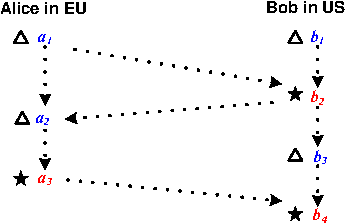
\includegraphics[width=0.9\columnwidth]{figures/redblue/redblueOrder/redblueGlobalOrder.pdf}
\label{fig:expositoryorder}
}
\end{minipage}
\par\bigskip
 \begin{minipage}[t]{0.5\columnwidth}
\centering
\subfloat[Causal serializations of $O$]{
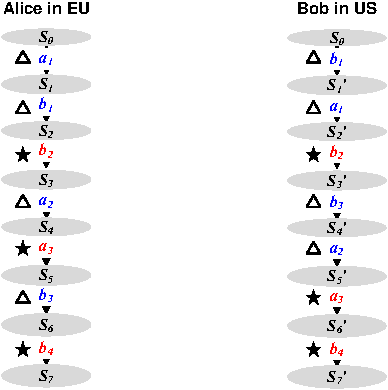
\includegraphics[width=1.0\columnwidth]{figures/redblue/redblueOrder/redblueOrderSerial.pdf}
\label{fig:expositoryexecutionorder}
}
\end{minipage}
\caption{\RBo\ and causal serializations for a system spanning two
  sites. \Operations\ marked with {\Large $\star$} are \red;
  \operations\ marked with $\bigtriangleup$ are \blue. Dotted arrows in \protect\subref{fig:expositoryorder} indicate
  dependencies between \operations. }
\label{fig:expositoryfigure}
\end{figure}

The definition of \RBc\ has two components:  
(1) A \RBo, which defines a (global) partial order of
\operations, and (2) a set of local causal
serializations, which define site-specific total orders
in which the \operations\ are locally applied.

\begin{mydef}[\RBo]
\label{def:rbo}
Given a set of \transactions\ $U=\R\cup \B$, where $\R\cap \B =
\emptyset$, a \emph{\RBo} is a partial order $O=(U,\prec)$ with the
restriction that $\forall u,v \in \R$ such that $u \neq v$, $u\prec v$
or $v\prec u$ (i.e., \red\ \operations\ are totally ordered).
\end{mydef}

Recall that each site is modeled as a deterministic state machine
capable of processing a totally ordered sequence of \operations. We
define which serializations are allowed for a given \RBo\ as follows:

\begin{mydef}[Legal serialization]
$O'=(U,<)$ is a {\em legal serialization} of \RBo\ $O=(U,\prec)$ if
\begin{itemize}
\item
$O'$ is a linear extension of $O$; i.e., $<$ is a total order
compatible with the partial order defined by $\prec$.
\end{itemize}
\label{def:legalserial}
\end{mydef}

This definition forces the serial order by which replicas execute
\operations\ to be compatible with the \RBo. However, it fails to
enforce causality, meaning that if an \operation\ $v$ sees the effects of \operation\ $u$ at its
primary site, then any \operation\ $w$ that sees the effects of $v$
must also see the effect of $u$ at all sites in the system.
In order to preserve causality, we extend the above
definition by saying that if \operation\ $v$ sees the effects of $u$
at its primary site, \site{v}, then  $u$ must be serialized before $v$ at all sites.

\begin{mydef}[Causal legal serialization]
  Given a site $i$, $O_i=(U,<)$ is an {\em $i$-causal legal serialization}
  (or short, a \emph{causal serialization}) of \RBo\ $O=(U,\prec)$ if
 \begin{itemize} 
  \item $O_i$ is a legal serialization of $O$, and 
  \item for any two \operations\ $u,v\in U$, if $\site{v}=i$ and $u<v$ in $O_i$, then
  $u\prec v$.
 \end{itemize}

\label{def:legalcausalserial}
\end{mydef}

A replicated system with
$k$ sites is then \RBct\ if every site applies a causal serialization
of the same global \RBo\ $O$.

\begin{mydef}[\RBc]
A replicated system is {\em $O$-\RBct} (or short, \RBct) if each site $i$ applies
operations according to an $i$-causal serialization of \RBo\ $O$.
\label{def:rbct}
\end{mydef}
%%%%%%%%% old version of the definition
\eat{
%\johannes{
\begin{mydef}[\RBc]
  A system is {\em $O$-\RBct} (or short, \RBct) if each site $i$ applies
operations according to an $i$-causal serialization of $O$.
%for all sites $i$, the state reached by site $i$ is the result of a
%site-$i$-causal serialization $O_i$ of the same \RBo\ $O$.
\label{def:rbct}
\end{mydef}
%}
}

Figure~\ref{fig:expositoryfigure} shows a \RBo\ and a pair of causal
serializations of that \RBo. In systems where every \operation\ is
labeled \red, \RBc\ is equivalent to
serializability~\cite{Bernstein1987CCR}; in systems where every
\operation\ is labeled \blue, \RBc\ allows the same set of behaviors as
causal consistency~\cite{Terry1995Managing,Lloyd2011Causal,
Mahajan2010Depot}. It is important to note that while \RBc\ constrains 
possible orderings of \operations\ at each site and thus the states the
system can reach, it does not ensure {\em a priori} that the system achieves 
all the end-to-end properties identified in Section~\ref{ch:redblue:sect:related}, 
namely, state convergence and invariant preservation, as discussed next.

\subsection{State convergence and a \RB\ bank}
\label{ch:redblue:sect:diverge}

In order to understand \RBc\ it is instructive to look at a concrete example. 
For this example, consider a simple bank with two users: Alice in the EU and Bob in the
US. Alice and Bob share a single bank account where they can deposit
or withdraw funds and where a local bank branch can accrue interest on
the account (pseudocode for the \operations\ can be found in
Figure~\ref{fig:bankPseudo}).  
Let the {\tt deposit} and {\tt accrueinterest} \operations\ be \blue.
Figure~\ref{fig:bankexample} shows a \RBo\ of deposits and interest
accruals made by Alice and Bob and two possible causal serializations applied at
both branches of the bank.

\begin{figure}[t]
\centering
\begin{minipage}{0.5\columnwidth}
%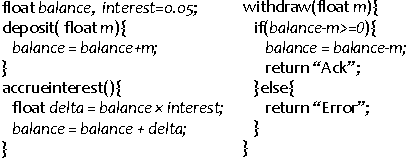
\includegraphics[width=1.0\columnwidth]{figures/redblueOrder/bankCode.pdf}
\pseudocodeinput[breaklines=true,mathescape=true]{pseudocode/redblue/basicexample.txt}
\end{minipage}
\caption{Pseudocode for the bank example.}
\label{fig:bankPseudo}
\end{figure}

\begin{figure}[t]
\centering
\begin{minipage}[t]{0.6\columnwidth}
\centering
\subfloat[\sf \RBo\ $O$ of \operations\ issued by Alice and Bob ]{
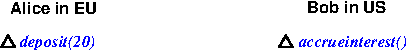
\includegraphics[width=0.9\columnwidth]{figures/redblue/redblueOrder/redblueOrderBank.pdf}
\label{fig:simplebankrbo}
}
\end{minipage}
\par\bigskip
\begin{minipage}[t]{0.6\columnwidth}
\centering
\subfloat[\sf Causal serializations of $O$ leading to diverged state]{
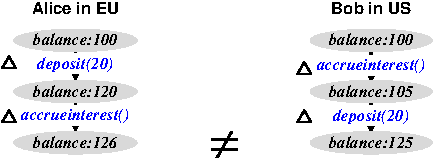
\includegraphics[width=1.0\columnwidth]{figures/redblue/redblueOrder/redblueOrderBankSerial.pdf}
\label{fig:divergestate}
}
\end{minipage}
\caption{A \RBct\ account with initial balance of \$100.}
% \changebars{and final diverged state}{}. \changebars{}{ (a) \RBo\ of
%  \operations\ issued by Alice and Bob. (b) Divergent causal serializations.}}
\label{fig:bankexample}
\end{figure}

State convergence is important for replicated systems. Intuitively a
pair of replicas is state convergent if, after processing the same
set of \operations, they are in the same state.  In the context of
\RBc\ we formalize state convergence as follows:

\begin{mydef}[State convergence]
A \RBct\ system is state convergent if all causal serializations of
the underlying \RBo\ $O$ reach the same state $S$ w.r.t any initial state $S_0$.
\end{mydef}

The bank example as described is not state convergent. The root cause is not surprising: \RBc\ allows
sites to execute \blue\ \operations\ in different orders but two
\blue\ \operations\ in the example correspond to non-commutative
operations---addition ({\tt dep\-osit}) and multiplication ({\tt accrueinterest}).
A sufficient condition to guarantee state convergence in a
\RBct\ system is that every \blue\ \operation\ is {\em globally commutative}, i.e., it commutes with all other
\operations, \blue\ or \red. We formally define this condition in the following
theorem.
%% \begin{theorem}
%%   For any \RBo\ $O=(U,\prec)$, if every 
%% %new
%% \changebars{\blue\ \operation\ is globally commutative, then $O$ is
%%   state convergent.}
%% %old
%% {pair of non-commutative \operations\ $u$ and $v$ are colored \red,
%%   then $O$ is state convergent.  }
%% %done
%% \footnote{All proofs will be found in a separated technical report,
%%   which is still under construction. \allen{This must be completed
%%     before we send the camera-ready.  EVen if it means simply
%%     uncommenting the text/proofs from the current TR forms}}
%% \label{them:commute}
%% \end{theorem}
%jg11: Suggest this new version of the theorem:

\begin{theorem}
Given a \RBo\ $O$, if all \blue\ \operations\ are globally commutative, then 
any $O$-\RBct\ system is state convergent.
\label{them:commute}
\end{theorem}

%%%%%new transition
In order to prove the above theorem, we introduce the following three lemmas along with 
their proofs.

The first lemma asserts that, given a legal serialization, swapping two
adjacent operations in the legal serialization that are not ordered by
the underlying \RBo\ results in another legal serialization.
\begin{lemma}\label{lem:canSwap}
Given a legal serialization $O_i=(U,<_i)$ of \RBo\ $O=(U,\prec)$
with \transactions\ $u,v\in U$ such that $u<_iv$ and $u \not\prec v$ and
there exists no $s$ such that $u<_{i}s<_{i}v$, and let $P=\{ p | p \in U \wedge p <_i u\}$
and $Q=\{q | q \in U \wedge v <_i q\}$. The serialization $O_k=(U,<_k)$ where
  \begin{itemize}
    \item $\forall p,q\in P \cup Q: p<_kq
      \Longleftrightarrow p<_iq$,
  \item $\forall p \in P: p <_k v$,
  \item $v<_k u$,
  \item $\forall q \in Q: u <_k q$
 \end{itemize}
 is a legal serialization.
 \end{lemma}

\noindent{\bf Proof:} It suffices to show that $\forall r,s \in U:$ $r<_k s$ is
   compatible with $\prec$. To do so, we consider the following six cases:

\begin{itemize}
\item {\bf Case 1:} $r,s\in P\cup Q$.  Since $O_i$ is a legal serialization,
each $r<_i s$ is compatible with $\prec$ by definition.  By
construction $\forall p,q\in P \cup Q:$ $r<_k s \Longleftrightarrow r<_i s$, so each $r<_k s$ is also compatible with $\prec$.

\item {\bf Case 2:} $r \in P$, $s = v$.  $r<_k s$ is compatible with $\prec$ by
similar logic as above.

\item {\bf Case 3:} $r = u$, $s \in Q$.  $r <_k s$ is compatible with $\prec$ by
 similar logic as above.

\item {\bf Case 4:} $v<_k u$.  Since $u\not\prec v$, $v<_k u$  is compatible with $\prec$. 

\item {\bf Case 5:} $r \in P$, $s = u$. Since $v <_{k} u \wedge \forall p \in P: p <_{k} v \implies p <_{k} u$. By the construction of $P$, $\forall p \in P: p <_{k} u \Longleftrightarrow p<_{i} u$. So each $r<_k s$ is also compatible with $\prec$.

\item {\bf Case 6:} $r = v$, $s \in Q$. Since $v <_{k} u \wedge \forall q \in Q: v <_{k} q \implies v <_{k} q$. $r <_k s$ is compatible with $\prec$ by
 similar logic as above.
\end{itemize}
As $U = P \cup Q \cup \{u,v\}$, by all above cases, $\forall r, s\in U:$ $r<_k s$ is compatible with $\prec$.\qed

%% Lemma 2: given a legal serialization and some pair of elements that
%% are unordered in the \rbo\, then there exists an adjacent pair of
%% elements that are not ordered.  (this ensures that the conditions for
%% lemma 1 are met)
The following lemma asserts that given a \RBo\ and its legal serialization, if there exists
a pair of elements that are not ordered by the \RBo, then there exists an adjacent
pair of elements between $u$ and $v$ in the legal serialization that are not ordered by the \RBo.

%The following lemma asserts that given two distinct legal
%serializations of the same \RBo, there exists an adjacent pair of
%operations in the first whose relative order in the second is
%reversed.

\begin{lemma}\label{lem:adjexists}
Given a legal serialization $O_i=(U,<_i)$ of \RBo\ $O=(U,\prec)$, if
$\exists u,v\in U$ such that $u<_i v$ and $u\not\prec v$,
let $U' = \{u,v\} \cup \{q|u<_i q\wedge q<_i v\}$, then $\exists r, s \in U'$ such that $r<_i s \wedge$ $r\not\prec s$ $\wedge \not\exists p \in U': r<_i p\wedge p <_i s$.
\end{lemma}
%% lemma 3: two legal serializations that differ in the order of one pair
%% of adjacent operations are convergent

\noindent{\bf Proof:}
We prove this by performing the following exhaustive analysis. The analysis
terminates when the required pair of elements is found.

Let's start with $u, v$. Consider $Q$ to be the sequence of elements strictly between $u$ and $v$, i.e.,
$Q=\{q\in U| u<_i q \wedge q <_i v\}$. There are two cases we have to analyze:
\begin{itemize}
\item {\bf Case 1:} $Q$ is empty. This implies that $u$ and $v$ are adjacent, so the analysis
terminates.

\item {\bf Case 2:} $Q$ is not empty. This implies that $u$ and $v$ are not adjacent.
Consider $p$ to be the first element in $U'$ according to $<_i$, i.e.,
$p\in U': \forall q\in U'\setminus\{p\}, p<_i q$. There are two cases to consider:
\begin{itemize}
\item {\bf Case 2a:} $u\not\prec p$. It follows that $p$ is the successor of $u$ in
$O_i$, then $u, p$ is the adjacent pair that are not ordered by $O$. The analysis
terminates.

\item {\bf Case 2b:} $u\prec p$. It follows from the assertion that $u\not\prec v$
and the transitivity of $\prec$ that $p\not\prec v$. Then we run
the analysis from the beginning with $p,v$. Since we are removing
the first element of the sequence $Q$, the analysis will either eventually
terminate with an empty sequence, or before that.
\end{itemize}
\end{itemize}
\qed


The third lemma asserts that two legal serializations that differ
in the order of exactly one pair of adjacent operations (one of which
is \blue) are state convergent, if all their \blue\ operations are globally
commutative.

\begin{lemma}\label{lem:adjacentconvergent}
Assume $O_i=(U,<_i)$ and $O_j=(U,<_j)$ are both legal
serializations of \RBo\ $O=(U,\prec)$ that are identical except for
two adjacent \transactions\ $u$ and $v$ such that $u<_iv$ and $v<_ju$ and that all
\blue\ operations $r\in U$ are globally commutative. Then
$S(O_i)=S(O_j)$.
\end{lemma}

\noindent{\bf Proof:} Let $P$ and $Q$ be the greatest common prefix and suffix
respectively of $O_i$ and $O_j$.  Further, let $S_P=S_0(P)$,
$S_{uv}=S_P+u+v$, and $S_{vu}=S_P+v+u$.

It follows from the definition of a \RBo\ (Definition~\ref{def:rbo}) and a legal serialization (Definition~\ref{def:legalserial})
that either $u\in B$ or $v\in B$.  Without loss of generality, assume
$u\in B$. By assumption $u$ commutes with all \transactions\ in $U$, therefore
$S_{uv}=S_{vu}$. It then follows the definition
of deterministic state machine that $S_{uv}(Q) = S_{vu}(Q)$. 
By the definition of legal serialization (Definition~\ref{def:legalserial}), 
the final state reached by sequentially executing operations in $O_{i}$ 
against $S$ according to $<$ is equal to the final state obtained by 
sequentially applying operations in $Q$ against $S_{uv}$ according to $<$, namely $S_0(O_i)=S_{uv}(Q)$. By
a similar argument, we know $S_0(O_j)=S_{vu}(Q)$. Finally, we have $S_0(O_i)=S_0(O_j)$.\qed


With the above lemmas, we could prove the state convergence theorem (Theorem~\ref{them:commute}) as follows:

\noindent{\bf Proof:} To prove a \RBct\ system is state convergent,
it is sufficient to show that for a \RBo\ $O$ of that system, any pair of its causal legal
serializations reaches the same final state w.r.t any initial state. To achieve
this, we take a slightly more conservative approach, which is to prove 
that any pair of legal serializations of their underlying \RBo\ $O$ is state convergent. 
Let $O_{i}$ and $O_{j}$ be two legal serializations of $O$. There are two cases to consider:

\begin{itemize}

\item {\bf Case 1:} $O_i = O_j$.  The underlying deterministic state
machine ensures that $S(O_i)=S(O_j)$.

\item {\bf Case 2:} $O_i \neq O_j$, in which case $\exists u,v\in U$
such that $u<_i v$ and $v<_j u$. Since both $O_i$ and $O_j$ are
legal serializations of $O$, it follows that $u\not\prec v$ and
$v\not\prec u$. It then follows Lemma~\ref{lem:adjexists} that we
can find an adjacent pair of operations $r, s$ such
that $r<_i s \wedge s<_j r \wedge r\not\prec s \wedge s\not\prec r$. We construct a new
serialization $O_{i+1}$ by first duplicating $O_i$ and then swapping the order of $r$ and $s$ in $O_{i+1}$, 
i.e., $r<_i s \wedge s<_{i+1} r$. By Lemma~\ref{lem:canSwap}, $O_{i+1}$ is 
also a legal serialization of $O$.

If $O_{i+1} \neq O_j$, we continue the construction by finding 
an adjacent pair of elements whose order is different in $O_{i+1}$, $O_j$. By swapping
the two operations, we obtain another legal serialization $O_{i+2}$. We can then continue to swap
all such adjacent pairs until the last constructed serialization
is equal to $O_j$. This is achievable since 
for any two legal serializations generated from two consecutive steps, $O'$ and $O''$,
the number of pairs in $O''$ whose orders
are different in $O_j$ becomes smaller than the number observed in $O'$.
At the end, the construction process results in a chain of legal
serializations where the first one is $O_i$ and the last is $O_j$, and any consecutive pair of legal serializations
is identical except for the order of an adjacent pair of elements. It then follows 
Lemma~\ref{lem:adjacentconvergent} and the assumption that
all \blue\ operations are globally commutative that every consecutive pair of
serializations in the chain is state convergent. Thus, $S_0(O_i)=S_0(O_j)$.\qed
\end{itemize}

Theorem~\ref{them:commute} highlights an important tension inherent to \RBc. On the one hand,
low latency requires an abundance of \blue\ \operations\ that can be
locally executed and lazily replicated. On the other hand, state
convergence requires that \blue\ \operations\ commute with all other
\operations, \blue\ or \red. In order to make the banking
example shown in Figure~\ref{fig:bankPseudo} and~\ref{fig:bankexample} converge, one has to label all three
operations \red, namely {\tt deposit}, {\tt withdraw} and {\tt accrueinterest}.
Obviously, this labeling will lead to a significant performance penalty, due
all operations must be serialized w.r.t each other. The poor result
implies that there exists an obstacle to making systems fast under \RBCN, which
is that the number of commuting operations in the real world is quite limited. 
As a result, in the following section
we introduce a method for addressing this tension by significantly
increasing the amount of commutativity in application \operations.
